For mobile and robotics applications a real-time encoder is needed. Hardware based real-time video encoders are expensive and not massively produced, thus their availability is limited. Creating one with off-the-shelf components opens the potential users. Two different models chosen whose computational cost was low enough to keep them operating at real-time and had kept biological plausibility constraints.


\subsection{The foveal pit model}

The highest resolution area of the eye is the foveal pit (see section \ref{sec:vision:eye}). A functional model for this region of the retina was developed by \citeauthor{basab-model}, they called the algorithm \emph{FoCal}\cite{basab-model}. It's based on the response and physiology of the fovea. The authors concluded that using four different layers of ganglion cells, most of the visually relevant information could be recovered after encoding. Furthermore, the encoder outputs a collection of rank-ordered spike trains. 

The ganglion cells where modelled using Difference of Gaussians (DoG), Equation \ref{eq-dog}. 

\begin{equation}
\label{eq-dog}
DoG_w(x,y) = \pm\frac{1}{2\pi\sigma_{w,c}^2}e^{\frac{-(x^2 + y^2)}{2\sigma_{w,c}^2}}
\mp\frac{1}{2\pi\sigma_{w,s}^2}e^{\frac{-(x^2 + y^2)}{2\sigma_{w,s}^2}}
\end{equation}

Each simulated cell type has a different scale $w$, which is reflected in the convolution kernel width. Variables $\sigma_{w,c}$ and $\sigma_{w,s}$ are the standard deviation for the centre and surround components of the DoG at scale $w$.  The signs for the equation will be ($-$,$+$) if the ganglion cell is \emph{off-centre} and ($+$,$-$) if it is \emph{on-centre}. The parameters for this equation can be found in table \ref{tab-kernel-specs}.

\begin{table}[htb]
  \caption{Simulation parameters for ganglion cells}
  \centering
  \bgroup
  \def\arraystretch{1.4}
  
  %  \begin{TAB}(r,1em,1.5em){|c|c|c|c|c|}{|c|c|c|c|c|} 
  \begin{tabular}{l c c c c}
    \begin{minipage}{3cm}Cell type \end{minipage}& 
    \begin{minipage}{1cm} \centering Matrix width \end{minipage}&  
    \begin{minipage}{2.5cm}\centering Centre \\std. dev. ($\sigma_c$)\end{minipage} & 
    \begin{minipage}{2.5cm}\centering Surround \\std. dev. ($\sigma_s$)\end{minipage} & 
    \begin{minipage}{2.5cm}\centering Sampling resolution \\(cols, rows)\end{minipage} \\
    \hline
    \begin{minipage}{3cm}\vspace*{0.1cm} Midget Off-centre \vspace*{0.005cm} \end{minipage}& 
    \begin{minipage}{0.5cm}\centering$3$ \end{minipage}& 
    $0.8$ & $6.7 \times \sigma_c$ & 1, 1\\
    \begin{minipage}{3cm} Midget On-centre \vspace*{0.005cm}\end{minipage} & 
    \begin{minipage}{0.5cm}\centering $11$ \end{minipage}& 
    $1.04$ & $6.7 \times \sigma_c$ &  1, 1\\
    \begin{minipage}{3cm}Parasol Off-centre \vspace*{0.005cm}\end{minipage} & 
    \begin{minipage}{1cm}\centering $61$ \end{minipage}& 
    $8$ & $4.8 \times \sigma_c$ & 5, 3 \\
    \begin{minipage}{3cm} Parasol On-centre \vspace*{0.005cm}\end{minipage} & 
    \begin{minipage}{0.5cm}\centering $243$\end{minipage} &
    $10.4$ & $4.8 \times \sigma_c$ & 5, 3
  \end{tabular}
  \label{tab-kernel-specs}
  \egroup
  \vspace*{-5pt}
\end{table}

For each cell type, a convolution kernel must be computed. For each element of the kernel we use Equation \ref{eq-dog} substituting parameters specified in Table \ref{tab-kernel-specs} and integer valued coordinates whose origin is the centre of the kernel. For example, for the Midget Off-centre type ($3\times3$ kernel), the upper-left value would be calculated as follows:

\begin{align}
\label{eq-dog-3x3}
DoG_3(x,y) &= -\frac{1}{2\pi\sigma_{3,c}^2}e^{\frac{-(x^2 + y^2)}{2\sigma_{3,c}^2}}
+ \frac{1}{2\pi\sigma_{3,s}^2}e^{\frac{-(x^2 + y^2)}{2\sigma_{3,s}^2}} \\
DoG_3(-1,-1) &= -\frac{1}{2\cdot\pi\cdot 0.8^2}e^{\frac{-((-1)^2 + (-1)^2)}{2\cdot 0.8^2}}
+ \frac{1}{2\cdot\pi\cdot 5.36^2}e^{\frac{-((-1)^2 + (-1)^2)}{2\cdot 5.36^2}} \nonumber \\[0.5em]
             &= 0.27399398 \nonumber
\end{align}

The procedure to encode images can be broken into two separate algorithm. On the first part (Algorithm \ref{code-focal-conv}), which simulates the ganglion cells, requires four independent convolutions using DoG kernels calculated as explained in the previous paragraph. 

\begin{algorithm}[h]
  \caption{FoCal, Part 1}
  \label{code-focal-conv}
  \begin{algorithmic}
    \Procedure{Convolution}{image $I$, kernels $K$}
    \State $C \leftarrow \emptyset$
    \ForAll{$k \in K$}
    \State $C \leftarrow C \cup convolution(k, I)$
    \EndFor
    \EndProcedure
    \algstore{bkbreak}
  \end{algorithmic}
\end{algorithm}

We'll call \emph{coefficients} $c_{i}$ to the pixels that come out of the convolutions. This coefficients should be interpreted as a quantity that is inversely proportional to the spike emission time. That is, the pixel with the largest coefficient value represents the ganglion cell that will spike first. 

The resulting coefficients from convolution happen to encode redundant information, because the DoG kernels are not an orthogonal basis. The eye does not output unnecessary information, lateral inhibition takes care of redundancy correction. It's still a matter of discussion where and by which cells is lateral inhibition performed in the retina. It is most likely to happen in layers prior to the ganglion cell layer. To correct for redundancy, FoCal performs a second step (Algorithm \ref{code-focal-corr}).

\begin{algorithm}[h]
  \caption{FoCal, Part 2}
  \label{code-focal-corr}
  \begin{algorithmic}
    \algrestore{bkbreak}
    \Procedure{Correction}{coeffs $C$, correlations $Q$}
    \State $N \leftarrow \emptyset$ \Comment{Corrected coefficients}
    \Repeat
    \State $m \leftarrow max(C)$
    \State $M \leftarrow M \cup m$
    \State $C \leftarrow C \setminus m$
    \ForAll{$ c \in C$} \Comment{Adjust all remaining c}
    \If{$Q(m, c) \neq 0$} \Comment{Adjust only near}
    \State $c \leftarrow c - m \times Q(m, c)$
    \EndIf
    \EndFor
    \Until{$C = \emptyset$}
    \State \textbf{return} $M$
    \EndProcedure
  \end{algorithmic}
\end{algorithm}

All the coefficients that where obtained from Algorithm \ref{code-focal-conv}, are put in a set $C$. For every step of the correction procedure the maximum coefficient is searched and its spatially surrounding pixels in all layers (Figure \ref{fig:focal2}) will be adjusted according to a the correlation between the maximum coefficient's convolution kernel and the other layers ones.

\begin{figure}
  \label{fig:focal2}
  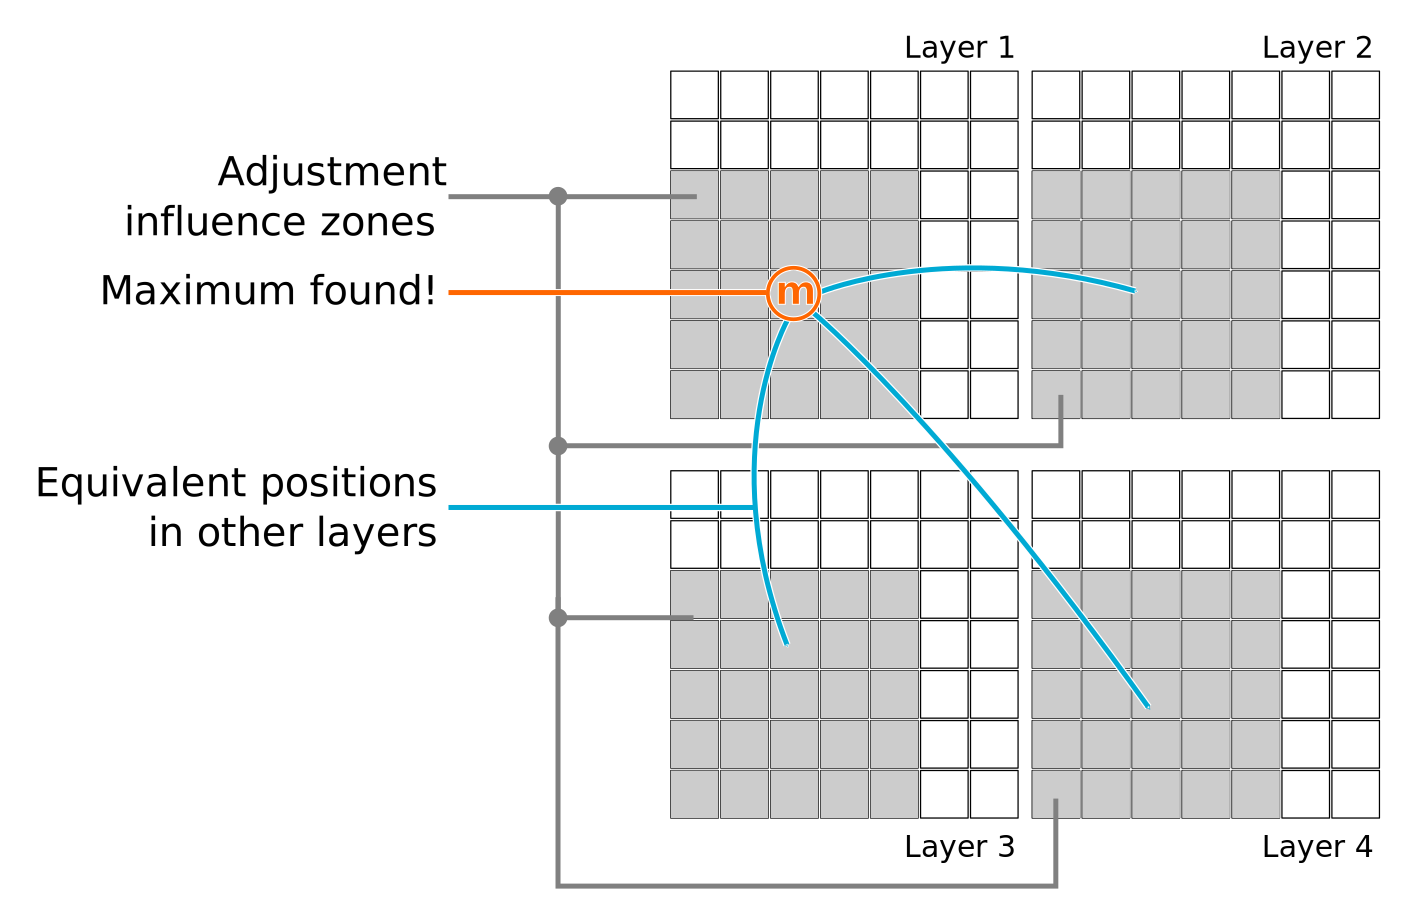
\includegraphics[width=\textwidth]{correction_adjustment}
  \caption{FoCal correction influence zones.}
\end{figure}



\begin{figure}[hbt]
  \centering
  \begin{subfigure}[t]{0.32\textwidth}
    \centering
    \captionsetup{justification=centering,margin=0.1cm}
    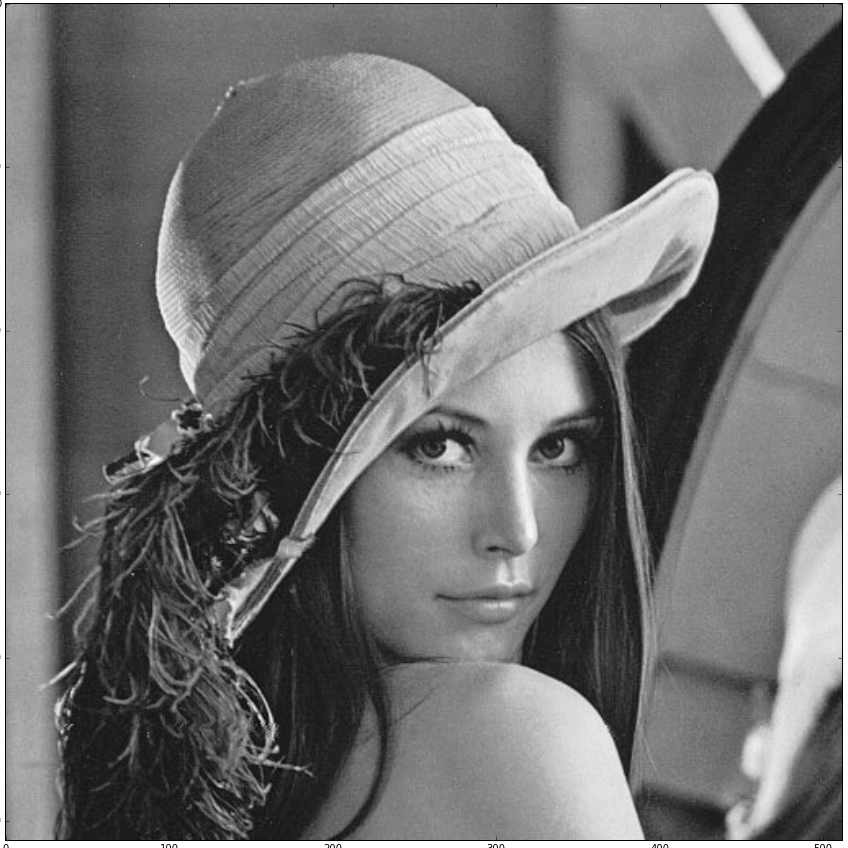
\includegraphics[width=\textwidth]{./Lena-gray}
    \caption{Original image}
    \label{pic-lena}
  \end{subfigure}
  \begin{subfigure}[t]{0.32\textwidth}
    \centering
    \captionsetup{justification=centering,margin=0.1cm}
    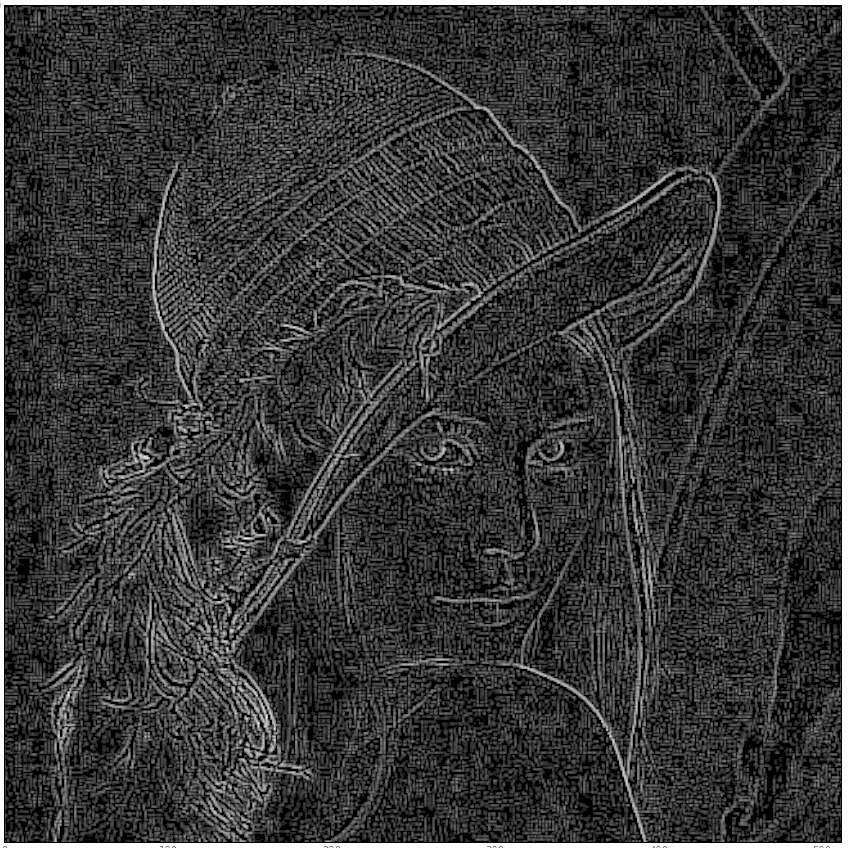
\includegraphics[width=\textwidth]{./Lena-midget_off}
    \caption{Midget OFF-centre}
    \label{pic-lena-M-OFF}
  \end{subfigure}
  \begin{subfigure}[t]{0.32\textwidth}
    \centering
    \captionsetup{justification=centering,margin=0.1cm}
    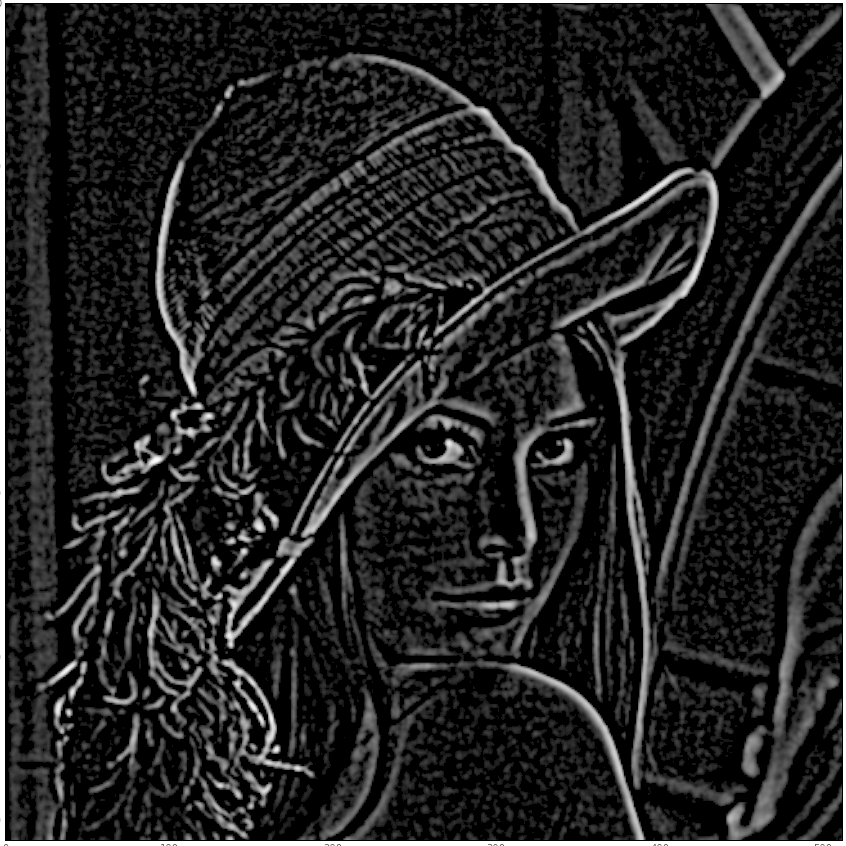
\includegraphics[width=\textwidth]{./Lena-midget_on}
    \caption{Midget ON-centre}
    \label{pic-lena-M-ON}
  \end{subfigure}
  \begin{subfigure}[t]{0.32\textwidth}
    \vspace*{0.8em}
    \centering
    \captionsetup{justification=centering,margin=0.1cm}
    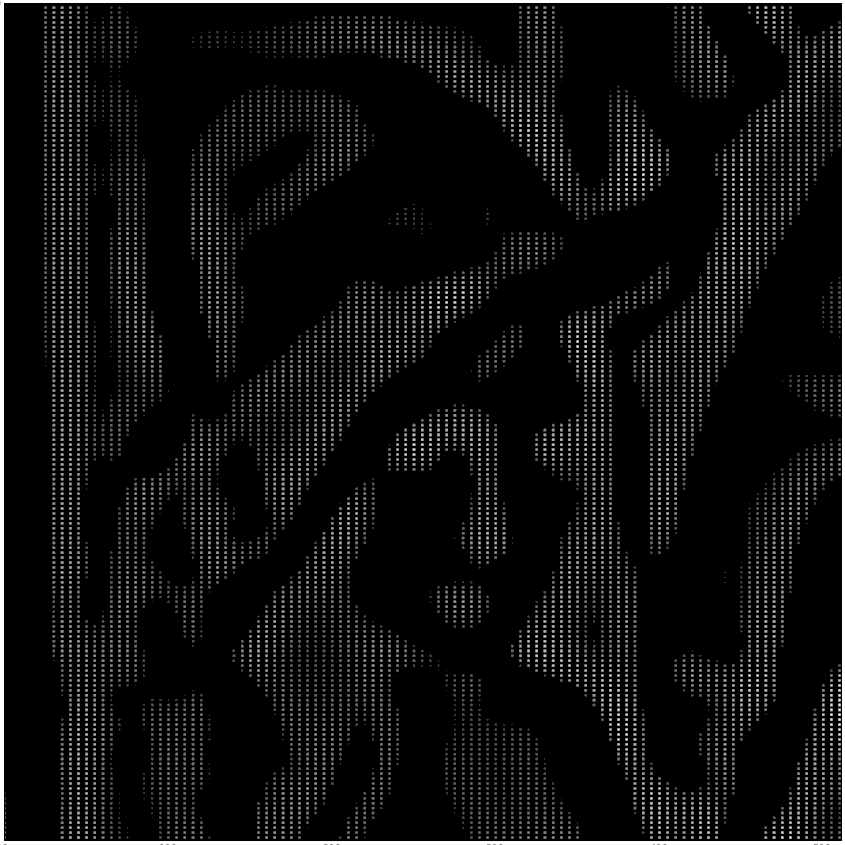
\includegraphics[width=\textwidth]{./Lena-parasol_off}
    \caption{Parasol OFF-centre}
    \label{pic-lena-P-OFF}
  \end{subfigure}
  \begin{subfigure}[t]{0.32\textwidth}
    \vspace*{0.8em}
    \centering
    \captionsetup{justification=centering,margin=0.1cm}
    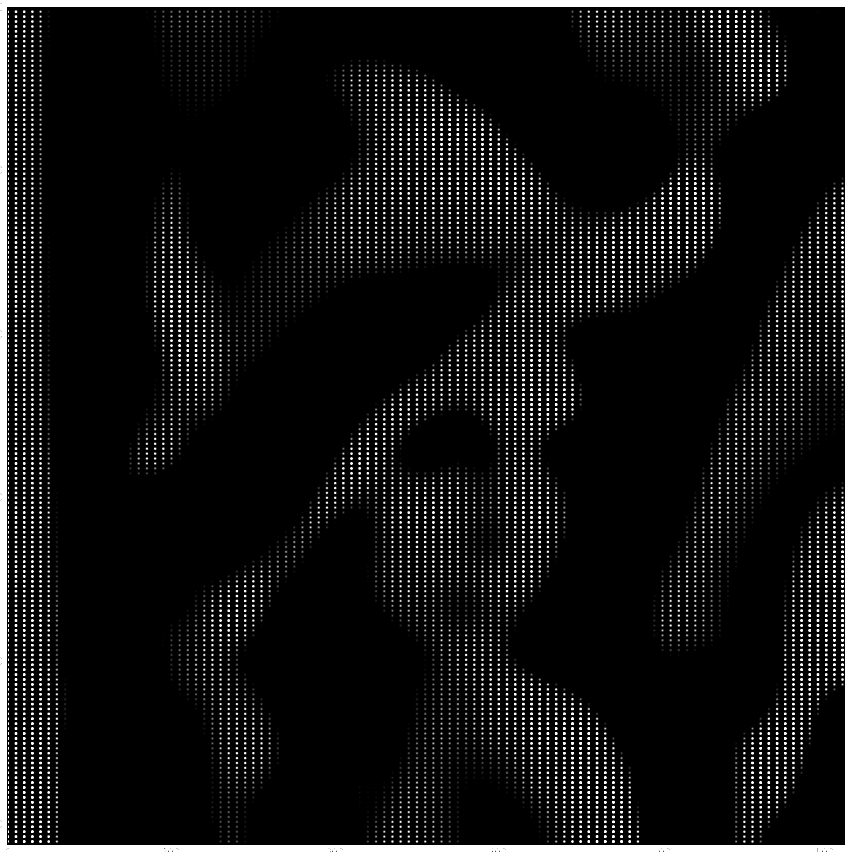
\includegraphics[width=\textwidth]{./Lena-parasol_on}
    \caption{Parasol ON-centre}
    \label{pic-lena-P-ON}
  \end{subfigure}
  \caption{Results of simulating ganglion cells (convolved images are enhanced for better contrast)}
  \label{fig-convolution-results}
\end{figure}
Every pixel in the convolved images (Fig.~\ref{fig-convolution-results}) 
represents a spike emission time, the higher the pixel value, the sooner the 
spike will be sent out.

Different ways of performing convolutions on a GPU where implemented, the naïve
does a discrete convolution with the full kernels; for the biggest kernel 
($243\times243$ elements) we were unable to fit it into one of the fast memory
locations of the GPU. We decompose the DoG into two horizontal and two vertical
convolution kernels to perform a separated convolution. This method works best 
on kernels bigger than $3\times3$. The last approach, \emph{Tiled Convolution} 
is reported by Advanced Micro Devices (AMD)~\cite{tiled-convolution}. They only 
present kernels of size $3\times3$, but we have an $11\times11$ convolution 
working; we are still developing solutions for the larger kernels.
Convolution alone is a compute intensive task and we 
obtain about 12 frames-per-second (FPS) on videos with $640\times360$ 8-bit 
grayscale pixel resolution. Encoding was carried out using a desktop computer 
running 64-bit GNU/Linux, with a Core i5-4570 4-core CPU @ 3.20~GHz processor 
with 8~GBytes of 64-bit DDR3 RAM @ 1600~MHz and a GeForce GT 720 GPU with 192 
CUDA cores @ 797~MHz, 1~GBytes of 64-bit DDR3 RAM @ 1800~MHz. %\\

\begin{table}
  \begin{center}
    \caption{Convolution performance comparison.}
    \bgroup
    \def\arraystretch{1.4}
    \begin{tabular}{l c c c c}
      &
      \begin{minipage}{2cm}\centering Midget\\Off-centre\vspace*{0.05cm}\end{minipage} & 
      \begin{minipage}{2cm}\centering
        Midget\\On-centre\vspace*{0.05cm}\end{minipage}& 
      \begin{minipage}{2cm}\centering
        Parasol\\Off-centre\vspace*{0.05cm}\end{minipage}& 
      \begin{minipage}{2cm}\centering
        Parasol\\On-centre\vspace*{0.05cm}\end{minipage}\\
      \hline 
      
      Naïve     & 0.0009s & 0.0031s & 0.0587s & N/A$^{1,2}$ \\ 
      Separated & 0.0021s & 0.0055s & 0.0172s & 0.0472s \\ 
      % x, y, 0.01756, 0.04500
      Tiled     & 0.0009s & 0.0044s & 0.1643 & N/A$^2$\\
    \end{tabular} 
    \egroup
    {
      \footnotesize 
      \begin{center}
        $^1$ Unable to fit convolution kernel into constant memory.\\
        $^2$ Unable to compile OpenCL code.
      \end{center}
    }
  \end{center}
  \vspace*{-5pt}
\end{table}

In the retina, redundancy of information is reduced via lateral inhibition 
prior to any ganglion cell activity. In this algorithm, we perform a correction 
on the convolved images by adjusting the pixel values
according to the correlation between convolution kernels 
(Alg.~\ref{code-focal-corr}). The results of using correction 
(Fig.~\ref{pic-unfiltered-spikes}) or not (Fig.~\ref{pic-100pc-spikes}) show 
that the convolution stage can only provide redundant information. Furthermore, 
using only 30\% of the corrected weights still provides enough visual 
information to reconstruct the original image~\cite{basab-model}.

\begin{figure}
  \centering
  \begin{subfigure}[t]{0.32\textwidth}
    \centering
    \captionsetup{justification=centering,margin=0.1cm}
    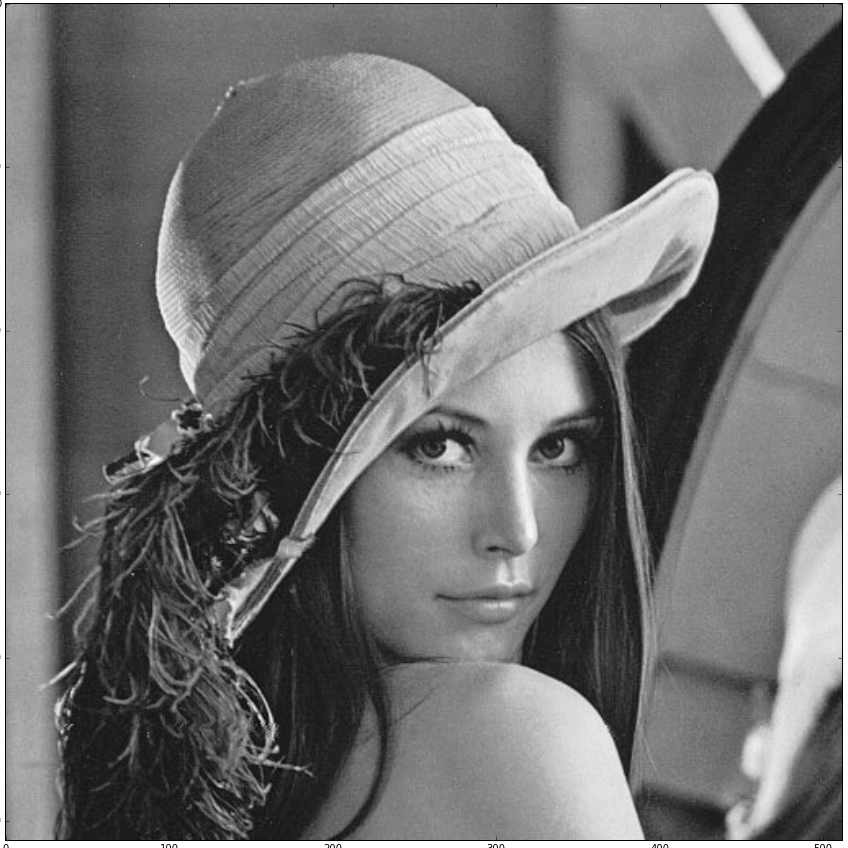
\includegraphics[width=\textwidth]{./Lena-gray}
    \caption{Original image}
    \label{pic-original-lena}
  \end{subfigure}
  \begin{subfigure}[t]{0.32\textwidth}
    \centering
    \captionsetup{justification=centering,margin=0.1cm}
    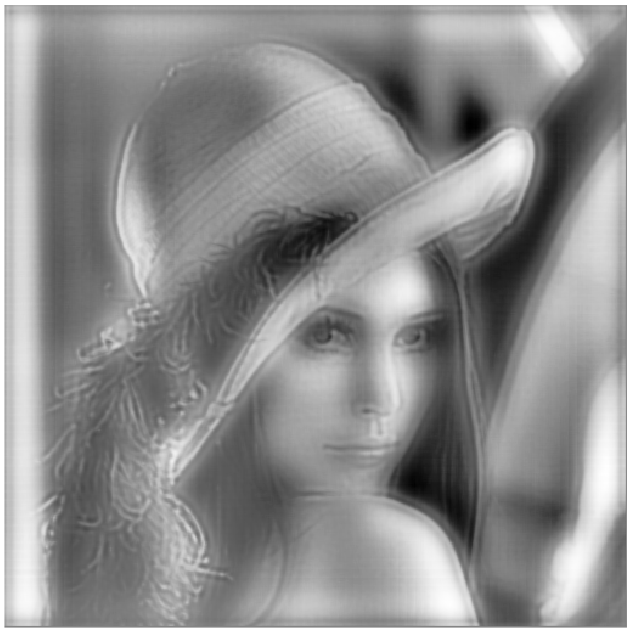
\includegraphics[width=\textwidth]{./final_results-unfiltered}
    \caption{100\% of raw spikes}
    \label{pic-unfiltered-spikes}
  \end{subfigure}
  %        \hfill
  \begin{subfigure}[t]{0.32\textwidth}
    \centering
    \captionsetup{justification=centering,margin=0.1cm}
    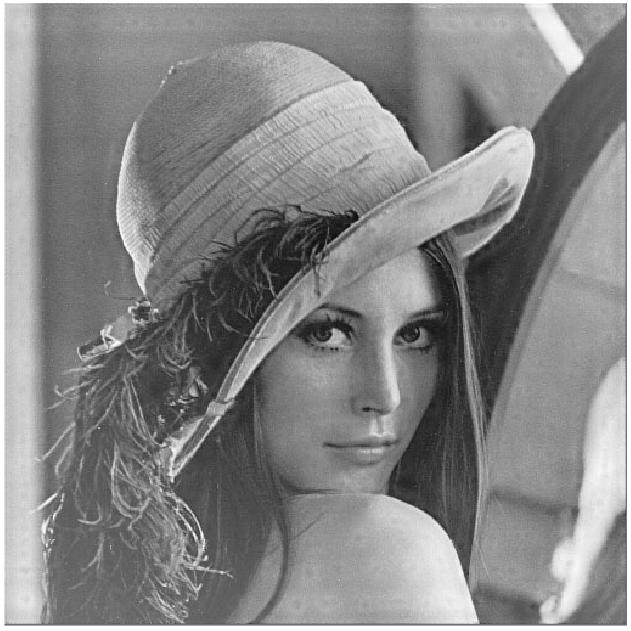
\includegraphics[width=\textwidth]{./final_results-focal-100}
    \caption{100\% of \emph{corrected} spikes}
    \label{pic-100pc-spikes}
  \end{subfigure}
  \caption{Results of reconstruction procedure}
  \label{fig-reconstruction}
  \vspace*{-10pt}
\end{figure}
Correcting the spikes for redundancy is a highly time consuming task which
might be better suited for event-based programming, such as the one found on 
the SpiNNaker platform. We are still working on an implementation for this 
approach.\\




12fps is for good most phenomenon, full image encoding

This probably happens only once every so many ms


\subsection{A dynamic vision sensor emulator}

Output what a DVS does but with a camera as a source

Convolution of current and past frames ? centre - current / surround - past

Per-pixel adaptive threshold keeps fast changing pixels from spiking constantly, emulates refractory period of cells.



A second way of encoding is to simulate the early stages of the retina, which 
sense changes in intensity on the photoreceptors. This is quite similar to what 
real Dynamic Vision Sensors (DVS) do but with limited dynamic range and lower 
temporal resolution~\cite{aer-retina-bernabe,dvs-zurich}. The main advantage is 
that no specialized hardware is needed and the operation is so fast that any 
recent computer should be able to do it. For this type of encoding procedure we 
hypothesize that the bigger the change, the sooner a cell would spike and, 
thus, we can obtain a spike timings given the difference of two video frames. 
So far we can process about 20 and 25 FPS using a Numpy and an OpenCL back-end, 
respectively (using the same hardware set-up previously described). Although 
it's currently a good approximation, more research on this algorithm is needed 
to better approximate to biology. 

